\section{Aufgabenstellung}
\label{sec:aufgabe}
Es soll ein Gerät entwickelt werden, das Bälle in einen Korb befördern kann.  
Das Spielfeld, auf dem die Aufgabe erledigt werden soll, ist dabei in 
\autoref{fig:playfield} dargestellt. Das Gerät befindet sich vor dem 
Startsignal im \mbox{\tikz{\draw[fill=yellow] (0,0) rectangle (0.25,0.25);} 
Startbereich} und darf die in \autoref{tab:device} definierten Abmessungen 
nicht überschreiten. Nach dem Startsignal darf sich der Roboter innerhalb von 
\mbox{\tikz{\draw[fill=yellow] (0,0) rectangle (0.25,0.25);} Start}- und 
\mbox{\tikz{\draw[fill=cyan] (0,0) rectangle (0.25,0.25);} Bewegungsbereich} 
bewegen. Der \mbox{\tikz{\draw[fill=red] (0,0) rectangle (0.25,0.25);} 
verbotene Bereich} darf jedoch weder berührt noch überragt werden. Im 
\mbox{\tikz{\draw[fill=green] (0,0) rectangle (0.25,0.25);} Zielbereich} 
befindet sich der Korb. Dieser wird erst direkt vor dem Startsignal platziert 
und muss vom Gerät  gefunden werden. Hinter dem Korb befindet sich eine Wand 
mit einer Höhe von 100 cm. Das Gerät muss die Aufgabe autonom absolvieren. 
\begin{figure}[h!]
    \centering
    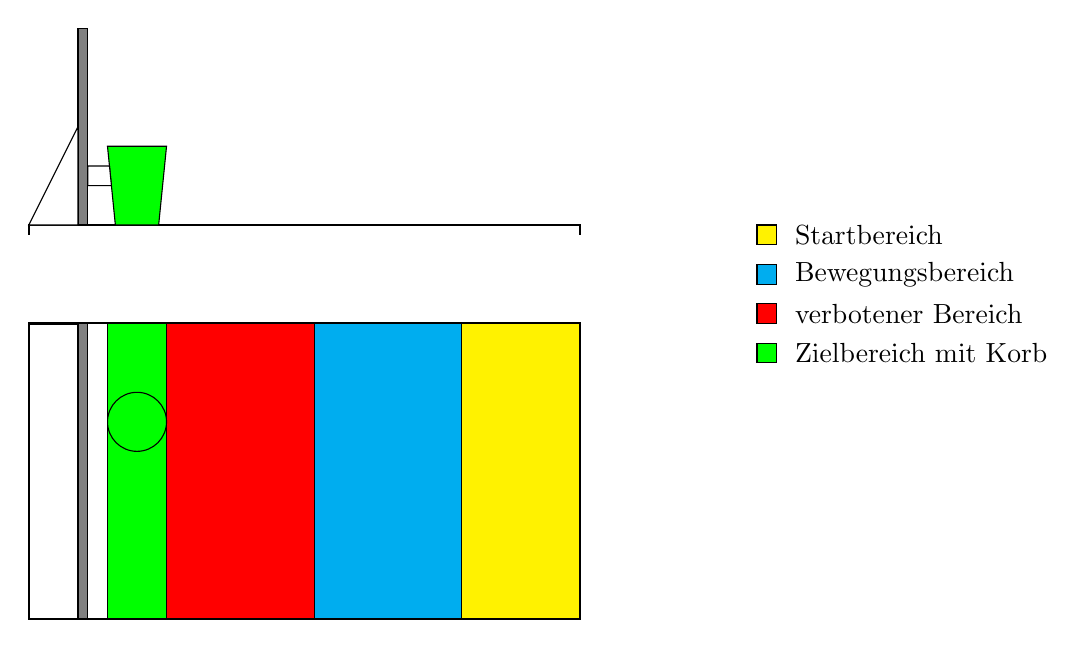
\begin{tikzpicture}[scale=0.025, rotate=90]
        \def \offset {200}          % Offset between Views of playfield
        \def \captionxoffset {130}  % Offset of caption in vertical distance
        \def \captionyoffset {-100} % Offset of caption in horizontal distance
        % playfield frame
        \draw[thick] (0,0) rectangle (150,280);
        \draw[thick] (\offset-5,0) -- (\offset,0) -- (\offset,280) -- (\offset-5,280);
        % startfield
        \draw[fill=yellow] (0,0) rectangle (150,60);
        % move field
        \draw[fill=cyan] (0,60) rectangle (150,135);
        % border line
        \draw[thick] (0,135) -- (150,135);
        % void field
        \draw[fill=red] (0,135) rectangle (150,210);
        % basket field
        \draw[fill=green] (0,210) rectangle (150,240);
        % basket
        \draw[fill=green] (100,225) circle [radius=15];
        \draw[fill=green] (\offset,214) -- (\offset+40,210) -- 
            (\offset+40,240) -- (\offset,236) -- (\offset,214);
        % gap filler
        \draw[fill=white] (0,240) rectangle (150,250);
        \draw[fill=white] (\offset+20,250) -- (\offset+20,238) -- (\offset+30,239) -- (\offset+30,250) -- (\offset+20,250);
        % wall
        \draw[fill=gray] (0,250) rectangle (150,255);
        \draw[fill=gray] (\offset,250) rectangle (\offset+100,255);
        \draw[fill=white] (\offset,255) -- (\offset+50,255) -- (\offset,280) -- (\offset,255);
        % caption
        \draw[fill=green]  (\captionxoffset+00,\captionyoffset) 
            rectangle node[right]{~ Zielbereich mit Korb}   
            (\captionxoffset+10,\captionyoffset+10);
        \draw[fill=red]    (\captionxoffset+20,\captionyoffset) 
            rectangle node[right]{~ verbotener Bereich}     
            (\captionxoffset+30,\captionyoffset+10);
        \draw[fill=cyan]   (\captionxoffset+40,\captionyoffset) 
            rectangle node[right]{~ Bewegungsbereich}       
            (\captionxoffset+50,\captionyoffset+10);
        \draw[fill=yellow] (\captionxoffset+60,\captionyoffset) 
            rectangle node[right]{~ Startbereich}           
            (\captionxoffset+70,\captionyoffset+10);
    \end{tikzpicture}
    \caption{Spielfeld}
    \label{fig:playfield}
\end{figure}

\noindent In diesem Kapitel werden die vorgegebenen Anforderungen an das Projekt 
besprochen. Dazu gehören Anforderungen an das Gerät sowie Rahmenbedingungen. 
In der Spalte Pflicht ist jeweils die Mindestanforderung beschrieben und in 
der Spalte Wunsch ist die vom Projektteam als Idealfall bezeichnete Leistung 
eingetragen. Zusätzlich wird eine Spalte Verantwortlichkeit angegeben. Hier
steht in Kurzform welcher Teilbereich von welcher Abteilung (Informatik, 
Elektrotechnik, Maschinenbau oder Dozenten) im Auge behalten werden muss.
\subsection{Gerät}
\begin{table}[h!]
    \centering
    \begin{zebratabular}[l]{@{}p{0.25\linewidth}p{0.3\linewidth}p{0.3\linewidth}p{0.07\linewidth}@{}}
        \rowcolor{gray} Anforderung &
            Pflicht &
            Wunsch &
            Verantw. \\
        Abmessungen & 
            $\leq$ 50 cm x 50 cm x 100 cm &
            &
            M \\
        Gewicht &
            &
            $\leq$ 2 kg &
            M, E \\
        Startbefehl &
            drahtlos &
            drahtlos von Handy &
            E, I \\
        Übermittlung Endsignal &
            An gleiches Gerät wie Startsignal &
            &
            E, I \\
        Aufhängevorrichtung &
            Kann von Federwaage gewogen werden &
            &
            M \\
        Design &
            &
            Optisch ansprechend &
            M \\
        Korbfindung &
            selbständig &
            &
            E, I \\
        Stromversorgung &
            &
            Interne Stromversorgung &
            E \\
    \end{zebratabular}
    \caption{Grundanforderungen aus Aufgabenstellung}
    \label{tab:device}
\end{table}

\clearpage
\subsection{Randbedingungen}
\begin{table}[h!]
    \centering
    \begin{zebratabular}[l]{@{}p{0.25\linewidth}p{0.3\linewidth}p{0.3\linewidth}p{0.07\linewidth}@{}}
        \rowcolor{gray} Anforderung &
            Pflicht &
            Wunsch &
            Verantw. \\
        Abmessungen Spielfeld &
            $\geq$ 148 cm x 58 cm &
            &
            Doz \\
        Freie Höhe über Spielfeld &
            $\geq$ 1.8 m &
            &
            Doz \\
        Freier Raum um Spielfeld &
            $\geq$ 0.5 m &
            &
            Doz \\
        Distanz Mittellinie bis Korb &
            75 cm $\ldots$ 1.9 m &
            &
            Doz \\
        Personensicherheit &
            muss jederzeit gewährleistet sein &
            &
            E, I, M \\
        Sicheres Beenden der Aufgabe &
            &
            ohne Beschädigung des Gerätes &
            I \\
        Not-Ausschalter &
            vorhanden &
            manuelle Steuerung &
            E, I \\
        Budget &
            $\leq$ 600 Fr. &
            &
            E, I, M \\
        Gewicht Tennisball &
            55 $\ldots$ 59 g &
            &
            Doz \\
        Durchmesser Tennisball &
            6.3 $\ldots$ 7.3 cm &
            &
            Doz \\
        Durchmesser Korb &
            30 cm &
            &
            Doz \\
        Höhe Korb &
            40 cm &
            &
            Doz \\
        Einrichtzeit &
            $\leq$ 5 min &
            $\leq$ 2 min &
            E, I, M \\
    \end{zebratabular}
    \caption{Randbedingungen aus Aufgabenstellung}
\end{table}

\clearpage
\subsection{Eigene Anforderungen}
Es werden noch spezifisch an Flug- beziehungsweise Bodenobjekte eigene 
Anforderungen gestellt. 

\subsubsection{Flugobjekt}
\begin{table}[h!]
    \centering
    \begin{zebratabular}[l]{@{}p{0.25\linewidth}p{0.3\linewidth}p{0.3\linewidth}p{0.07\linewidth}@{}}
        \rowcolor{gray} Anforderung &
            Pflicht &
            Wunsch &
            Verantw. \\
        Dauer zur Erfüllung der Aufgabe &
            $\leq$3 min &
            1 min &
            E, I, M \\
        Effizienz &
            5 Bälle im Korb &
            &
            E, I, M \\
        Abfluggewicht &
            $\leq$2 kg (ohne Bälle) &
            $\leq$1 kg (ohne Bälle) &
            E, M \\
        Funktional &
            Fokus auf Funktion &
            &
            E, I, M \\
        Design &
            Leichtbau &
            Ansprechendes Design &
            M \\
        Special-Effects &
            &
            Beim Abschlusssignal soll ein Special-Effect ausgelöst werden 
                (Konfetti, Rauch, Sound, usw.) &
            E, I, M \\
    \end{zebratabular}
    \caption{Eigene Anforderungen an ein Flugobjekt}
\end{table}

\subsubsection{Bodenobjekt}
\begin{table}[h!]
    \centering
    \begin{zebratabular}[l]{@{}p{0.25\linewidth}p{0.3\linewidth}p{0.3\linewidth}p{0.07\linewidth}@{}}
        \rowcolor{gray} Anforderung &
            Pflicht &
            Wunsch &
            Verantw. \\
        Dauer zur Erfüllung der Aufgabe &
            $\leq$3 min &
            1 min &
            E, I, M \\
        Effizienz &
            min. 3 Bälle im Korb &
            5 Bälle im Korb &
            E, I, M \\
        Gewicht &
            $\leq$8 kg &
            $\leq$2 kg &
            E, M \\
        Design &
            Elegantes, spezielles Design &
            abheben von Konkurrenz &
            M \\
        Special-Effects &
            &
            Beim Abschlusssignal soll ein Special-Effect ausgelöst werden (Konfetti, Rauch, Sound, usw.) &
            E, I, M \\
    \end{zebratabular}		
    \caption{Eigene Anforderungen an ein Bodenobjekt}
\end{table}
